\documentclass[a4paper,12pt,titlepage]{article}
%\usepackage[T1]{fontenc}
\usepackage[utf8]{inputenc}
\usepackage{graphicx}
%\usepackage[italian]{babel}
\usepackage{amsmath}
\graphicspath{{./images/}}
\title{Riassunto Fisica Tecnica}
\author{Simone Tomè}
\begin{document}
\maketitle
%da fare indice%
\paragraph{Capitolo 1}
\section{Sistema termodinamico}
\subsection{Sistema Semplice}
Un sistema termodinamico semplice gode delle seguenti caratteristiche: 
\begin{itemize}
\item chimicamente e fisicamente omogeneo ed isotropo;\\
\item non soggetto a campi magnetici/gravitazionali;\\
\item esente da effetti di superficie;\\
\end{itemize} 
Un sistema all'equilibrio ìè descritto da un numero di variabili termodinamiche che possono essere \textbf{estensive} (dipendenti dall'estensione/massa del sistema) o \textbf{intensive}. Il numero di variabili intensive utilizzabili per descrivere un determinato sistema è definito dalla \textbf{Regola di Gibbs}: \\
$V = C + 2 - F $ dove: C è il numero di componenti che compongono il sistema (se fosse composto esclusivamente da contorno + acqua C = 1) e F è il numero di fasi del componente/i facente parte del sistema (liquido,gassoso,solido).
\subsection{Contorno del sistema}
\begin{center}
\begin{tabular}{c | c}
\hline
\textbf{Contorno} & \textbf{Caratteristiche} \\
\hline
adiabatico o isolante & impermeabile al calore \\
\hline
diatermano o conduttore & permeabile al calore \\
\hline
rigido & non scambia lavoro \\
\hline
deformabile o mobile & scambia lavoro \\
\hline
impermeabile & non scambia massa \\
\hline
poroso & permette lo scambio di massa \\
\hline 

\hline
\end{tabular}
\end{center}
\subsubsection{Sistema chiuso e aperto}
Un sistema è detto \textbf{chiuso} quando non permette scambi di massa con l'esterno, la massa del sistema ad un istante di tempo iniziale sarà quindi uguale a quella presente nell'istante finale considerato. Un sistema è invece \textbf{aperto} quando permette di scambiare massa con l'esterno (ad esempio una turbina). Un sistema è detto \textbf{isolato} quando non ho scambi energetici con l'esterno ed è un caso particolare del sistema chiuso.
\subsection{Trasformazione termodinamica}
In una trasformazione termodinamica il sistema passa da uno stato d'equilibrio ad un altro.
\begin{itemize}
\item \textbf{internamente reversibile}:
costituita da una successione di stati di equilibrio;
\item \textbf{reversibile}: percorsa in senso inverso riporta sistema e ambiente allo stato iniziale. Le int. rev. possono anche non essere reversibili. 
\item \textbf{irreversibili}: trasformazione in parte o per intero non reversibile. Non è rappresentabile su un diagramma di stato. Per comodità viene talvolta indicata sui diagrammi come una linea tratteggiata congiungente i due stati di equilibrio iniziale e finale (rappresentabili).
\item \textbf{chiusa/cilcica}: lo stato finale corrisponde a quello iniziale;
\item \textbf{elementare}: una grandezza rimane costante durante la trasformazione;
\end{itemize}

\subsection{Gas Ideali}

Dedotta dalla teoria cinetica dei gas ecco l'equazione dei gas ideali:
\begin{center}
$PV = NRT $ dove R è la costante dei gas : $R = 8314 \cfrac{J}{kmole * K}$
\end{center}
Forme alternative ricordando che $V = v*M$ e che $N = \cfrac{M}{M_{mol}}$
e \\ $R^{*} = \cfrac{R}{M_{mol}} \left[\cfrac{J}{kg*K}\right]$.\\
\begin{center}
$Pv = R^{*}T $\\ e \\
$Pv_{mol} = RT $ dove $v_{m}$ è $\cfrac{V}{N} \left[\cfrac{m^{3}}{kmole}\right]$
\end{center}

\subsection{Liquidi e solidi}

Faccio l'assunzione che nell'equazione f(P,v,T) = 0 ci sia il volume che assume il ruolo di variabile dipendente così da diventare v = v(P,T). Differenziando ottengo; \begin{center}
dv = $\left(\cfrac{\partial v}{\partial T}\right)_{P}$ dT +  $\left(\cfrac{\partial v}{\partial T}\right)_{T}$ dP
\end{center} 
Si definiscono ora i coefficienti termodinamici:
\begin{center}
$\beta = \cfrac{1}{v}\left( \cfrac{\partial v}{\partial T} \right) _{P}$ detto coeff. di dilatazione termica isobaro \\
$K_{T} = -\cfrac{1}{v}\left( \cfrac{\partial v}{\partial P} \right)_{T} $
detto coefficiente di comprimibilità isotermo.
\end{center}
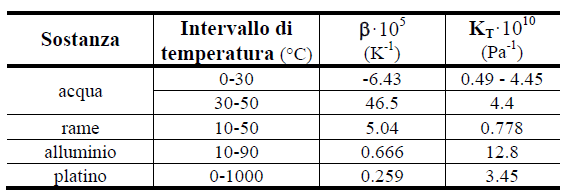
\includegraphics[scale=0.8]{Coefficienti}

Dalla formula precedente si possono ricavare le formule utili per la risoluzione di esercizi che trattano liquidi e solidi sapendo che:
\begin{center}
$ dv = \beta vdT - K_{T}vdP $
\end{center}

\paragraph{Capitolo 2}
\section{Principi di conservazione}
\subsection{Primo principio della termodinamica}
Il primo principio deriva dalla conservazione dell'energia di un sistema.\\
Per un sistema semplice all'equilibrio è definita una proprietà intrinseca (funzione di stato) detta energia interna U la cui variazione è il risultato di interazioni del sistema con l'ambiente esterno:
\begin{center}
$\varDelta U = Q^{\leftarrow}-L^{\rightarrow}$ 
\end{center}
dove $Q^{\leftarrow}$ è positivo se il calore è entrante nel sistema e
$L^{\rightarrow}$ è positivo se il lavoro è uscente dal sistema.\\
L'energia interna del sistema è una quantità estensiva quindi $U = M \times u$\\
Essendo una quantità estensiva se ho un sistema Z composto da più sottosistemi ho:
\begin{center}
$U_{Z} = U_{A} + U_{B} $
$\varDelta U_{Z} = \varDelta U_{A} + \varDelta U_{B}$
\end{center}
In un sistema isolato il bilancio deve essere nullo quindi $\varDelta U_{\text{isolato}} = 0$.\\
In un sistema che subisce una trasformazione ciclica essendo u funzione di stato ottengo che $\varDelta U = U_{f} - U_{i} = 0$ e quindi $Q^{\leftarrow} = L^{\rightarrow}$.\\

Con il termine di \textbf{lavoro termodinamico} l’energia fornita ad un sistema termodinamico semplice che sia riconducibile ad un processo di variazione di quota di un grave. Si definisce \textbf{calore} l’energia fornita ad un sistema termodinamico semplice e che non è riconducibile alla variazione di quota di un grave.\\
In forma differenziale e usando le grandezze specifiche il primo principio si scrive come:
\begin{center}
$du = \delta q^{\leftarrow} - \delta l^{\rightarrow}$
\end{center}
Sappiamo che l'energia interna è funzione di stato grazie all'esperienza di Joule che dimostra che l'energia interna per due stati di equilibrio è indipendente dal "percorso" compiuto dalla trasformazione per arrivare a quel determinato stato.

\subsection{Secondo Principio della termodinamica}
Il secondo principio colma le lacune del primo (verso delle reazioni spontanee e limite della trasformazione di calore in lavoro). Noi useremo la formulazione assiomatica del secondo principio.\\
In un sistema termodinamico all'equilibrio esiste una funzione intrinseca dello stato del sistema (funzione di stato) detta \textbf{entropia} S la cui variazione per una trasformazione reversibile è data da:
\begin{center}
$$ \varDelta S_{\text{rev}} = \int \cfrac{\delta Q_{\text{rev}}^{\leftarrow}}{T}  $$ 
\end{center}
L'entropia è una quantità estensiva e quindi gode delle proprietà viste per esse: additività e $S = M \times s$. \\
La variazione di entropia totale di un sistema isolato dove avvengono trasformazioni termodinamiche è sempre maggiore o uguale a zero. $$ \varDelta S \geq 0 $$, tende a 0 quando i processi sono reversibili. 
\clearpage
L'irreversibiltà genera entropia quindi:
\begin{center}
$ \varDelta S = S^{\leftarrow}= S^{\leftarrow}_{Q} + S_{\text{irr}}$
\end{center}

\paragraph{Capitolo 3}
\section{Grandezze Termodinamiche}
\subsection{Lavoro}
Il lavoro è definito come la forza per lo spostamento. In un sistema cilindro/pistone:\\
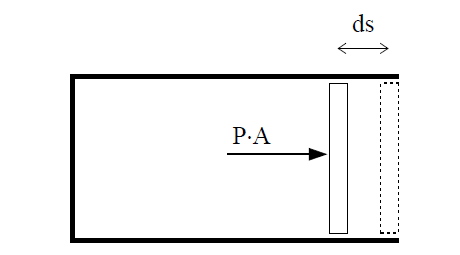
\includegraphics[scale=0.5]{work_piston}
\begin{center}
$ \delta L^{\rightarrow} = P  A ds = P dV $
\end{center}
Usando le grandezze specifiche: 
\begin{center}
$\delta l^{\rightarrow} = Pdv$
\end{center}
Il lavoro scambiato durante la trasformazione diventa quindi: 
\begin{center}
$$l = \int^{f}_{i}Pdv $$
\end{center}
Il lavoro a livello grafico è l'area sottostante alla curva della trasformazione nel grafico Pv.\\
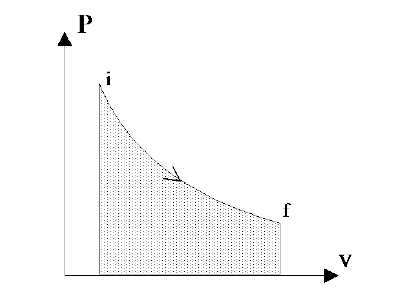
\includegraphics[scale=0.5]{work_Pv}
\clearpage
Il lavoro non è funzione di stato poichè \textbf{dipende} dalla trasformazione. In caso di una trasformazione \textbf{ciclica} se il ciclo viene percorso in senso orario il lavoro uscente è maggiore di zero, altrimenti il lavoro uscente dal sistema risulta negativo.
\subsection{Calore}
Si definisce capacità termica Cx il rapporto tra il calore fornito al sistema termodinamico e la variazione di temperatura del sistema stesso:
\begin{center}
$C_{x} = \left( \cfrac{\delta Q^{\leftarrow}}{dT} \right)_{x} $
\end{center}
dove il pedice precisa la trasformazione lungo la quale avviene lo scambio di calore.\\
Calore specifico: $$ c_{x} = \cfrac{1}{M} \left( \cfrac{\delta Q ^{\leftarrow}}{dT}  \right)_{x} = \cfrac{C_{x}}{M}$$
Di particolare interesse sono $c_{v}$ e $c_{p}$ che possono essere interpretati come derivate parziali (primo principio).
\begin{center}
$$\delta q^{\leftarrow} = du +Pdv  $$
$$\delta q^{\leftarrow} = \left( \cfrac{\partial u}{\partial T} \right)_{v}dT + 
\left( \cfrac{\partial u}{\partial V} \right)_{T}dv + Pdv$$
\end{center}
A volume costante (dv = 0) ho quindi:
\begin{center}
$$\left( \cfrac{\delta q^{\leftarrow}}{dT} \right)_{v}
=  \left( \cfrac{\partial u}{\partial T} \right)_{v} = c_{v} $$
\end{center}
\clearpage
\subsection{Entalpia}
La funzione (di stato) \textbf{entalpia} è definita come:
\begin{center}
h = u + Pv = H/M
\end{center} 
Differenziando:
\begin{center}
dh = du + vdP +Pdv
\end{center}
Ricordando il primo principio:
\begin{center}
dh = $\delta $q$^{\leftarrow}$ + vdP
\end{center}
Per una trasformazione isobara ho quindi: 
\begin{center}
$$\left( \cfrac{\delta q^{\leftarrow}}{dT} \right)_{P}
=  \left( \cfrac{\partial h}{\partial T} \right)_{P} = c_{P} $$
\end{center}
\subsection{Relazione di Mayer}
Manipolando algebricamente i differenziali di c$_{v}$ e c$_{P}$ trovati (pressione e volume costante), definizione della funzione entalpia e la legge dei gas ideali trovo la seguente relazione detta di Mayer:
\begin{center}
c$_{P}$ = c$_{v}$ + R$^{*}$
\end{center}
\begin{itemize}
\item \textbf{Gas monoatomico} $$c_{v} = \cfrac{3}{2}R^{*}$$
\item \textbf{Gas biatomico o poliatomico lineare} $$c_{v} = \cfrac{5}{2}R^{*}$$
\item  \textbf{Gas poliatomico non lineare} $$c_{v} = \cfrac{6}{2}R^{*}$$
\end{itemize}
Per un \textbf{liquido incomprimibile ideale}  c(T)$ = $c$_{v} = $c$_{p}$, per un \textbf{liquido incomprimibile perfetto} è anche costante e non varia in base alla temperatura.
\subsection{Trasformazioni politropiche}
Ricordo che per un gas ideale valgono le seguenti:
\begin{center}
du = c$_{v}$ dT\\
dh = c$_{p}$ dT\\
$\delta$q$^{\leftarrow}$ = c$_{x}$ dT 
\end{center}
Sostituendo i valori nelle equazioni del primo principio ed entalpia: 
\begin{center}
$\delta$q$^{\leftarrow}$ = du + Pdv \\
$\delta$q$^{\leftarrow}$ = dh - vdP
\end{center}
Ottengo questa relazione:
\begin{center}
$\cfrac{c_{x}-c_{P}}{c_{x}-c_{v}}=- \cfrac{vdP}{Pdv} = n$
\end{center}
La \textbf{trasformazione politropica} è una trasformazione quasi-statica per un gas ideale dove questa relazione è costante ed è chiamata \textbf{indice della politropica} (indicato con la lettera $n$).\\
Separando le variabili e integrando ottengo:
\begin{center}
$$\int\cfrac{ndv}{v}=-\int\cfrac{dP}{P}$$\\
$lnv^{n} = -lnP + c$\\ 
$$Pv^{n} = c$$ dove $c$ è una costante
\end{center}
Ricordando la formula dei gas perfetti e che NR è costante, ottengo:
\begin{center}
$Pvv^{n-1} = costante$ $\rightarrow$ $Tv^{n-1} = costante$\\
$T\left( \cfrac{R^{*}T}{P} \right)^{n-1} = costante$ $\rightarrow$ $\cfrac{T^{n}}{P^{n-1}}=PT^{\frac{n}{1-n}} =costante$\\
\end{center}
La costante n assume valori diversi in base alla trasformazione presa in considerazione e questo influisce sulla forma del lavoro considerato. \\
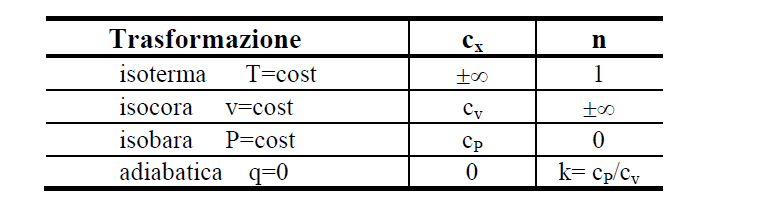
\includegraphics[scale=0.5]{cp_cvPNG}
\subsection{Espressioni per il lavoro}
Manipolando l'integrale del lavoro con le eqazioni trovate prima per la politropica ottengo che:
\begin{center}
$$ l = \cfrac{P_{1}v_{1}}{n-1}\left[ 1- \left( \cfrac{v_{1}}{v_{2}} \right)^{n-1} \right]
$$
$$
l = \cfrac{P_{1}v_{1}}{n-1}\left[ 1- \left( \cfrac{P_{2}}{P_{1}} \right)^{\frac{n-1}{n}} \right]
$$
\end{center}
\begin{itemize}
\item \textbf{Isobara n=0}: $$ l=P_{1}v_{1}ln\cfrac{v_{2}}{v_{1}} $$ 
\item \textbf{Isoterma n=1}: $$ l=P_{1}v_{1}ln\cfrac{P_{1}}{P_{2}} $$
\end{itemize}
\subsection{Entropia e diagramma T-S}
In un diagramma T-S l'area sottostante la curva che rappresenta una trasformazione \textbf{reversibile} rappresenta il calore scambiato durante la trasformazione essendo:
\begin{center}
$dS_{rev} = \cfrac{\delta Q_{rev}}{T}$ $\rightarrow$ $Q_{rev} = \int T(S)dS_{rev} $\\
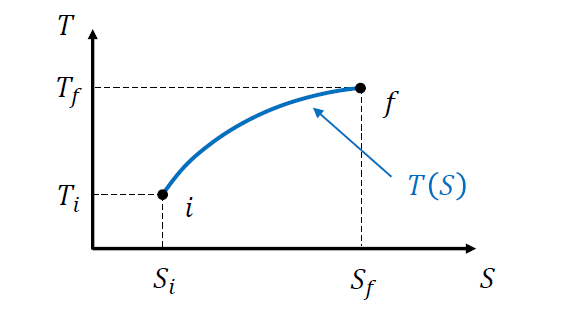
\includegraphics[scale=0.5]{t-s_diagram}
\end{center}

Per una trasformazione \textbf{ciclica} internamente reversibile , le aree incluse
nelle curve chiuse rappresentative del ciclo nei diagrammi P-V e T-S sono uguali , essendo, per il primo principio:
$ \varDelta U = 0$  $\rightarrow$  $Q^{\leftarrow} = L^{\rightarrow}$
\begin{center}
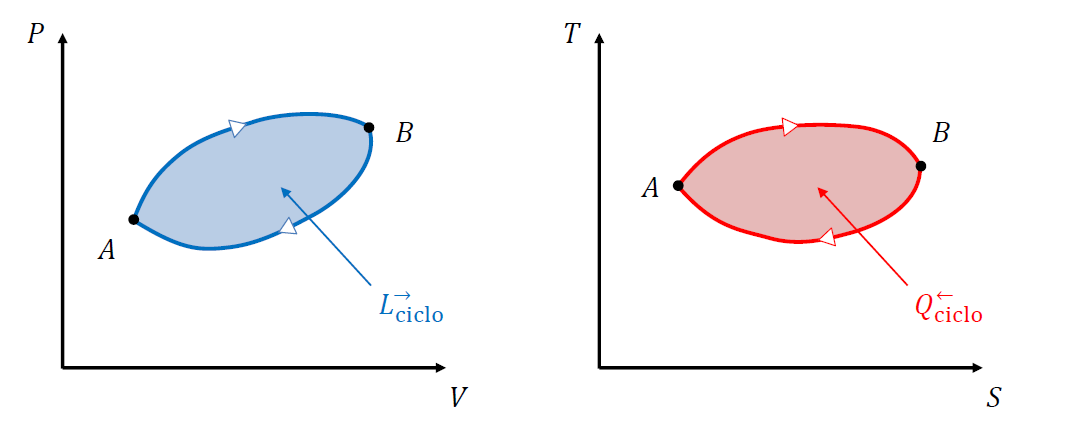
\includegraphics[scale=0.4]{cycle_same_q_l}
\end{center}
In un processo reversibile ho che il \textbf{primo principio} si può scrivere come:
\begin{center}
du = dsT - Pdv $\rightarrow$ ds = $\cfrac{du}{T} + \cfrac{Pdv}{T}$
\end{center}
Nell'ipotesi che il sistemi sia costituito da un \textbf{gas ideale} abbiamo che:
\begin{center}
du = c$_{v}$dT $\rightarrow$ ds = $c_{v}\cfrac{dT}{T} + R^{*}\cfrac{dv}{v}$
\end{center}
equivalentemente:
\begin{center}
ds = $c_{p}\cfrac{dT}{T} - R^{*}\cfrac{dP}{P}$\\
ds = $c_{p}\cfrac{dv}{v} + c_{v}\cfrac{dP}{P}$
\end{center}
Integrando (con ipotesi di c costanti) ottengo quindi:
\begin{center}
$ s = s_{0} + c_{v}ln\cfrac{T}{T_{0}} + R^{*}ln\cfrac{v}{v_{0}}$ \\
$ s = s_{0} + c_{P}ln\cfrac{T}{T_{0}} - R^{*}ln\cfrac{P}{P_{0}}$ \\
$ s = s_{0} + c_{P}ln\cfrac{T}{T_{0}} + c_{v}ln\cfrac{P}{P_{0}}$
\end{center}
Nel caso di \textbf{liquido incomprimibile ideale} e perfetto ottengo che:
\begin{center}
ds = c$\cfrac{dT}{T} $ $\rightarrow$ s = s$_{0}$ + cln$\cfrac{T}{T_{0}}$
\end{center}
Ricordo che \textbf{l'entropia è funzione di stato} e quindi tra gli stessi estremi di una trasformazione $\varDelta$S è identica per le due trasformazioni. 
\clearpage
\paragraph{capitolo 4}
\section{Sistemi eterogenei}
\subsection{Grandezze estensive}
Un sistema si definisce \textbf{eterogeneo} quando i suoi componenti sono a diversi stati di aggregazione.
Essendo il sistema eterogeneo questo incide sulle \textbf{grandezze estensive}. \\
Sia $E$ una grandezza estensiva del sistema ed $e$ la corrisponte specifica. Consideriamo un sistema bifase monocomponente (due stati di aggregazione), allora:
\begin{center}
$M = M_{1}+M_{2}$ 


$$E = M \times e = \sum{M_{i}} \times e $$ 

$$e = \cfrac{M_{1}}{M}e_{1} + \cfrac{M_{2}}{M}e_{2}$$
\end{center}
dove il rapporto tra le masse è definita come \textbf{frazione massica} $x_{i}$.
Quindi:
\begin{center}
$$ \cfrac{M_{1}}{M} = x_{1}; \;\;\; \cfrac{M_{2}}{M} = x_{2} $$
$$ x_{1} + x_{2} = 1$$
$$ e = (1-x_{2})e_{1} + x_{2}e_{2}$$
\end{center}

\clearpage
\subsection{Funzione di stato}
Per un sistema bifase monocomponente ho bisogno di una coppia di variabili intensiva-estensiva per la \textbf{regola di Gibbs}. \\
Per vedere lo stato di aggregazione in cui si trova un componente posso usare il diagramma di stato (P-V-T):
\begin{center}
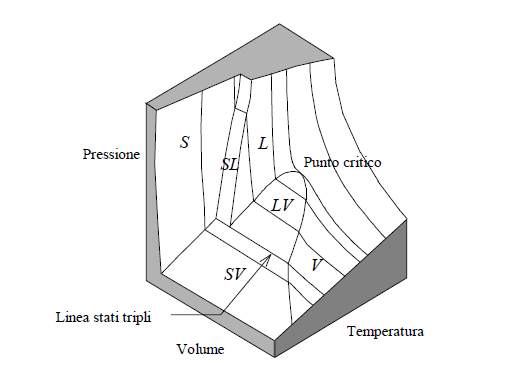
\includegraphics[scale=0.5]{state_diagram}\\
\end{center} 
In questo diagramma di stato si è preso in considerazione una sostanza che solidificandosi riduce il proprio volume specifico.La definizione di temperatura critica precisa che la isoterma critica è tangente alla curva limite in un punto chiamato \textbf{punto critico}. In corrispondenza del punto critico anche le altre variabili termodinamiche assumeranno un preciso valore caratteristico della particolare sostanza (pressione critica Pcr, volume critico vcr, etc.).
\begin{center}
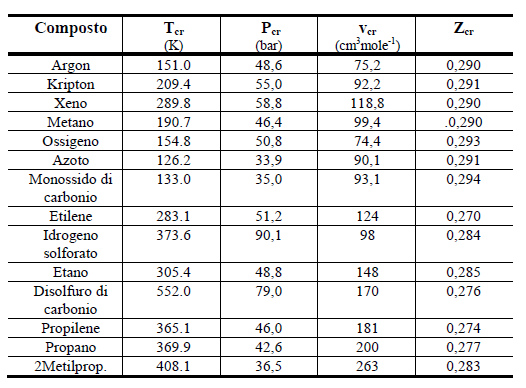
\includegraphics[scale=0.9]{tcr}

\end{center}
\clearpage
Nel diagramma esistono zone dove coesistono due stati di aggregazione, dal punto di vista ingegneristico quella più importante è quella dove coesiste lo stato liquido e vapore (liquido/vapore saturo).

\subsection{Passaggio di stato}
Proiettando il diagramma P-V-T su un piano di sole due coordinate ottengo un diagramma dove posso vedere, fissata una variabile, come devono variare le altre due per avere una transizione di stato.
\begin{center}
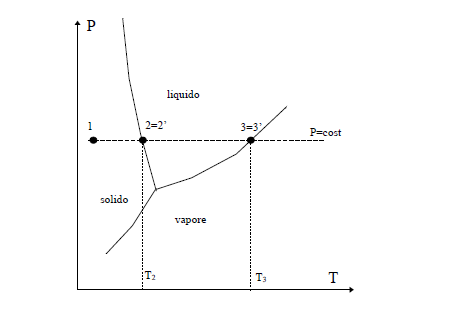
\includegraphics[scale=0.6]{state_trans}
\end{center}
Il punto di convergenza delle tre linee è detto \textbf{punto triplo} e coesistono i diversi stati di aggregazione della materia. Ricordando che:
\begin{center}
dh = dq + vdP $\;\;\;\;\rightarrow \;\;\;\;$ $h_{sol}<h_{liq}<h_{vap}$
\end{center}
Durante una transizione di stato pressione e volume sono costanti quindi $$dh = \delta q^{\leftarrow}$$
Per gli stati bifase non posso usare il piano P-T per la regola di Gibbs che richiede o una terna oppure una coppia con una variabile estensiva.
 
\subsection{Sistemi bifase liquido-vapore}
Sia x il \textbf{titolo vapore} ovvero $\cfrac{M_{v}}{M}$ allora come già visto:
\begin{center}
s = (1-x)s$_{l}$ + x$\,$s$_{v}$ \\
u = (1-x)u$_{l}$ + x$\,$u$_{v}$ \\
h = (1-x)h$_{l}$ + x$\,$h$_{v}$ \\
v = (1-x)v$_{l}$ + x$\,$v$_{v}$ \\
\end{center}
\clearpage
\begin{itemize}
\item \textbf{liquido sottoraffreddato}: liquido non in procinto di evaporare (L);
\item \textbf{liquido saturo}: liquido in procinto di evaporare;
\item \textbf{vapore saturo}: vapore in procinto di condensare;
\item \textbf{vapore surriscaldato}: vapore non in procinto di condensare (V);
\item \textbf{Temperatura di saturazione}: temperatura alla quale una sostanza pura comincia ad evaporare/condensare,
fissata la pressione;
\end{itemize}
Diagramma T-s:
\begin{center}
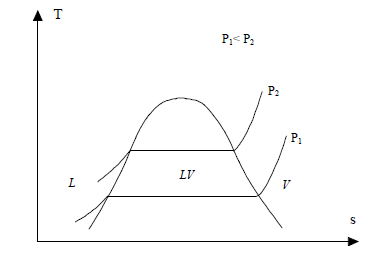
\includegraphics[scale=0.8]{t_s_graph}
\end{center}
Le linee orizzontali sono dette \textbf{isotermobariche} e sapendo che:
\begin{center}
dh = Tds + vdP
\end{center}
Se P costante: $ T = \cfrac{dh}{ds}$

\subsection{Interpolazione lineare}
Usando le tabelle a volte non ho i dati necessari, ma posso conoscerne uno e da quello estrarne un'altro facendo un'ipotesi di linearità della funzione:
\begin{center}
$$ Y = Y_{A} + \cfrac{Y_{B}-Y_{A}}{X_{B}-X_{A}}(X-X_{A})$$ con $\;\;\;X_{A}<X<X_{B}$
\end{center}

\subsection{Relazioni semplificate}
Usando il punto triplo dell'acqua posso ottenere i valori delle funzioni di stato h-s usando trasformazioni isobare e isoterme:
\begin{center}
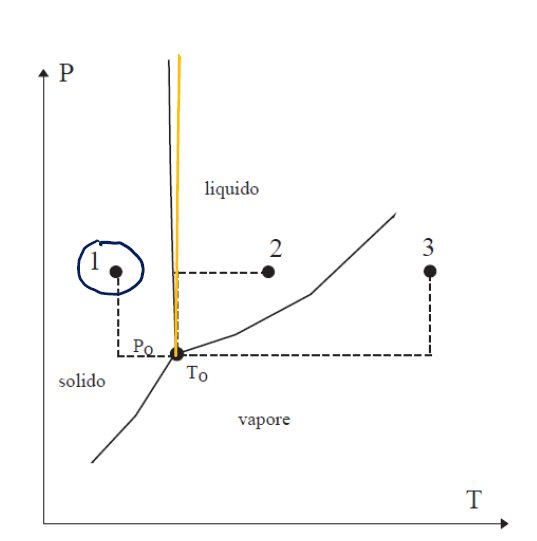
\includegraphics[scale=0.45]{p_t}
\end{center}
\begin{itemize}
\item \textbf{solido}:
Approssimando T0 a Tsat$_(L-S)$(P)
\begin{center}
$h(P,T) = h_{0} + h_{lst} +c_{s}(T-T_{0}) + v_{s}(P-P_{0}) $\\
$s(P,T) = s_{0}+s_{lst}+c_{s}ln\cfrac{T}{T_{0}} =  s_{0}+\cfrac{h_{lst}}{T_{0}}+c_{s}ln\cfrac{T}{T_{0}} $
\end{center}
\item \textbf{liquido}:
\begin{center}
$h(P,T)=h_{0}+c_{l}(T-T_{0}) +v_{l}(P-P_{0}) $\\
$ s(P,T) = s_{0}+c_{l}ln\cfrac{T}{T_{0}}$ 
\end{center}
\item \textbf{vapore}:
\begin{center}
$h(P,T)=h_{0}+h_{lvt} +c_{p}(T-T_{0}) $\\
$s(P,T) = s_{0}+s_{lvt}+c_{p}ln\cfrac{T}{T_{0}} - R^{*}ln\cfrac{P}{P_{0}} =  s_{0}+\cfrac{h_{lvt}}{T_{0}}+c_{p}ln\cfrac{T}{T_{0}}  - R^{*}ln\cfrac{P}{P_{0}} $
\end{center}
\end{itemize}
Con: 
\begin{itemize}
\item $P_{0}$ e $T_{0}$ pressione e temperatura del punto triplo (0.00611 bar e 0.01 gradi celsius);
\item $h_{0}$ e $s_{0}$ entalpia ed entropia del punto triplo in fase liquida = 0 kJ/kg(h) e 0 kJ/kgK (s)
\item $h_{lst}$ entalpia di solidificazione del pt = -333 kJ/kg
\item $c_{s}$ : calore specifico del ghiaccio =2093 J/kgK
\item $v_{s}$: volume specifico del ghiaccio =0.00109 m$^3$/kg
\item $c_{l}$: calore specifico dell’acqua liquida =4186 J/kgK
\item  $v_{l}$: volume specifico dell’acqua liquida =0.001 m$^3$/kg
\item $h_{lvt}$ : entalpia di evaporazione al punto triplo = 2501.6 kJ/kg
\item $c_{p}$: calore specifico a pressione costante dell’acqua vapore =2009 J/kgK
\end{itemize}

\subsection{Formule per l'acqua sottoraffreddata}
Modello di liquido incomprimibile ideale:
$$dh = c(T)dT+vdP $$
$$ds = c(T)\cfrac{dT}{T}$$
Ricordo che per uno perfetto c è costante (posso integrare le variabili ottendendo $\varDelta s$ e $\varDelta h$):
\begin{center}
$\varDelta s = c\varDelta T + v\varDelta P$\\
$\varDelta s = cln\cfrac{T_{2}}{T_{1}}$
\end{center}
Per calcolare l'entropia di un liquido (incomprimibile ideale) sottoraffreddato partendo dalla curva di saturazione e utilizzando una trasformazione isoterma:
$$h(P,T)-h_{ls}(P_{sat}(T))= c(T-T)+v(P-P_{sat}) = h_{ls}(P_{sat}(T)) +v(P-P_{sat}) $$
dove posso usare $v = v_{ls}(P_{sat(T)})$.\\
Quest'ultimo termine è solitamente trascurabile.
\begin{center}
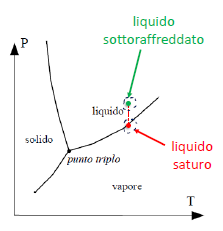
\includegraphics[scale=0.6]{p_t_liquido_sottoraffreddato}
\end{center}



\end{document}